\section{Interface 1}

On considère le problème à l'interface 1 uniquement (voir figure~\ref{iface1}).

\begin{figure}[!h]
    \centering{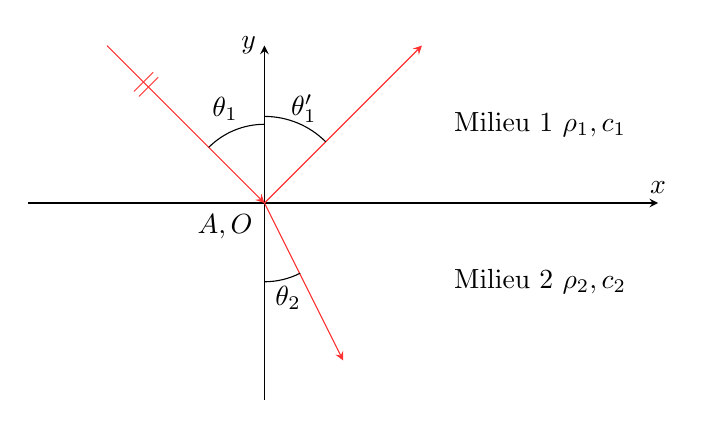
\begin{tikzpicture}

    % ifaces
    \draw [>=stealth, ->] (-3,0) -- (5,0);

    % Labels
    \draw (3.5,1) node {Milieu 1 $\rho_1,c_1$};
    \draw (3.5,-1) node {Milieu 2 $\rho_2,c_2$};

    % verticals
    \draw [dashed] (0,1.5) -- (0,-1.5);

    % axis
    %% y
    \draw [>=stealth, ->] (0,-2.5) -- (0,2);
    \draw (-.2,2) node {$y$};
    %% x (already drawn)
    \draw (5,.2) node {$x$};


    % points A & B
    \draw (-.5, -.3) node {$A,O$};

    % rays
    \draw [red!80, >=stealth, ->] (-2,2) -- (0,0) node[near start, sloped] {$| |$};
    \draw [red!80, >=stealth, ->] (0,0) -- (2,2);
    \draw [red!80, >=stealth, ->] (0,0) -- (1, -2);

    % angles
    \draw (0,1) arc (90:135:1) node at (-0.5,1.2) {$\theta_1$};
    \draw (0,1.1) arc (90:45:1.1) node at (0.5,1.2) {$\theta_1'$};
    \draw (0,-1) arc (-90:-63:1) node at (0.3,-1.2) {$\theta_2$};

\end{tikzpicture}
}
    \caption{\label{iface1} Considération des effets à l'interface 1}
\end{figure}

\subsection{Position du problème}


\paragraph{Pressions totales} Dans le milieu 1, la pression totale vérifie :

\begin{equation}
    \left(\Delta - \frac{1}{c_1^2}\frac{\partial^2}{\partial t^2}\right)\pTOT_1(x,y,t) = 0 \;;\; \forall x,t \,\mathrm{et}\, \forall y \geq 0 \label{i1_prop1}
\end{equation}


Dans le milieu 2, la pression totale vérifie :

\begin{equation}
    \left(\Delta - \frac{1}{c_2^2}\frac{\partial^2}{\partial t^2}\right)\pTOT_2(x,y,t) = 0 \;;\; \forall x,t\,\mathrm{et}\,\forall y \leq 0 \label{i1_prop2}
\end{equation}


\paragraph{Champ monochromatique} Les ondes sont considérées monochromatiques, l'équation d'Helmholtz est donc vérifiée
dans chacun des milieux :

\begin{eqnarray}
    (\Delta + k_1^2)p_1(x,y) & = & 0 \;;\; \forall x,t \label{i1_helm1}\\
    (\Delta + k_2^2)p_2(x,y) & = & 0 \;;\; \forall x,t \label{i1_helm2}
\end{eqnarray}

On définit les nombres d'onde $k_i = \nicefrac{\omega_i}{c_i}$, $\omega_i$ étant la pulsation de l'onde dans le milieu
$i$ ($i\in \{1,2\}$).

\paragraph{Condition de Sommerfeld}

\paragraph{Conditions à l'interface}

A l'interface, il y a continuité des pressions et des vitesses normales. Ainsi :

\begin{eqnarray}
    \pTOT_1(x, y=0, t) &=& \pTOT_2(x,y=0,t) \;;\;\forall x,t \label{i1_cl1}\\
    \vTOT_1(x, y=0, t) &=& \vTOT_2(x,y=0,t) \;;\;\forall x,t \label{i1_cl2}
\end{eqnarray}

Dans le milieu 2, on ne considérera que l'onde transmise, ainsi pour les equations~\eqref{i1_prop2},~\eqref{i1_cl1}
et~\eqref{i1_cl2}, on aura :

\begin{eqnarray*}
    \pTOT_2 = \pT_1\\
    \vTOT_2 = \vT_1
\end{eqnarray*}

On définit alors :

$$\pTOT_1 = \pI_1 + \pR_1$$

\subsection{Forme générale des pressions}

Les ondes sont considérés monochromatiques :

\begin{eqnarray}
    \pI_1(x,y,t) & = & A_1e^{j(\omega_1t-k_1\sin\theta_1x+k_1\cos\theta_1y)} \label{i1_pgeni}\\
    \pR_1(x,y,t) & = & B_1e^{j(\omega_1t-k_1\sin\theta_1'x+k_1\cos\theta_1'y)} \label{i1_pgenr}\\
    \pT_1(x,y,t) & = & A_2e^{j(\omega_2t-k_2\sin\theta_2x+k_2\cos\theta_2y)} \label{i1_pgent}
\end{eqnarray}

\subsection{Forme générales des vitesses normales}

On sait que les vitesses normales ont une expression de la forme : $v_i(x,y,t) = v_i(x,y)e^{j\omega_it}$, d'après
l'équation d'Euler, on peut écrire les équations~\eqref{i1_euler1} et \eqref{i1_euler2}.

\begin{eqnarray}
    \rho_1\frac{\partial\vTOT_1}{\partial t} = -\frac{\partial\pTOT_1}{\partial y}
        & \Leftrightarrow & \vTOT_1 = -\frac{1}{j\omega_1\rho_1}\frac{\partial\pTOT_1}{\partial y}\label{i1_euler1} \\
    \rho_2\frac{\partial\vT_1}{\partial t} = -\frac{\partial\pT_1}{\partial y}
        & \Leftrightarrow & \vT_1 = -\frac{1}{j\omega_2\rho_2}\frac{\partial\pT_1}{\partial y}\label{i1_euler2}
\end{eqnarray}

De l'équation~\eqref{i1_euler1} on peut déduire la forme de $\vTOT_1$ (équation~\eqref{i1_vgentot}), et
de~\eqref{i1_euler2} on déduit~\eqref{i1_vgent}.

\begin{eqnarray}
    \vTOT_1
        & = & -\frac{1}{j\rho_1\omega_1}\left[ jA_1k_1\cos\theta_1e^{j(\omega_1t-k_1\sin\theta_1x+k_1\cos\theta_1y)} -
            jB_1k_1\cos\theta_1'e^{j(\omega_1t-k_1\sin\theta_1'x-k_1\cos\theta_1'y)}\right]\notag\\
        & = & -\frac{1}{\rho_1\omega_1}\left[A_1k_1\cos\theta_1e^{j(\omega_1t-k_1\sin\theta_1x+k_1\cos\theta_1y)} -
            B_1k_1\cos\theta_1'e^{j(\omega_1t-k_1\sin\theta_1'x-k_1\cos\theta_1'y)}\right] \label{i1_vgentot}
\end{eqnarray}

\begin{eqnarray}
    \vT_1
        & = &
    -\frac{1}{j\rho_2\omega_2}\left[jA_2k_2\cos\theta_2e^{j(\omega_2t-k_2\sin\theta_2x+k_2\cos\theta_2y)}\right]\notag\\
        & = &
    -\frac{1}{\rho_2\omega_2}\left[A_2k_2\cos\theta_2e^{j(\omega_2t-k_2\sin\theta_2x+k_2\cos\theta_2y)}\right]
    \label{i1_vgent}
\end{eqnarray}

\subsection{Conditions aux limites}

\subsubsection{Continuité des pressions}

On a 

\begin{equation*}
\eqref{i1_cl1} \Leftrightarrow \pTOT_1(x,y=0,t) = \pT_1(x, y=0 t) \;;\; \forall x,t 
\end{equation*}

Ainsi, en insérant~\eqref{i1_pgeni},~\eqref{i1_pgenr} et~\eqref{i1_pgent} dans~\eqref{i1_cl1}, on obtient
l'équation~\eqref{i1_cl1_insert}.

\begin{eqnarray}
    A_1e^{j\omega_1t}e^{-jk_1\sin\theta_1x} + B_1e^{j\omega_1t}e^{-jk_1\sin\theta_1'x} & = & A_2e^{j\omega_2t}e^{-jk_2\sin\theta_2x} \label{i1_cl1_insert}
\end{eqnarray}

On veut que~\eqref{i1_cl1_insert} soit valable pour tout $t$, on a alors :

\begin{eqnarray}
    e^{j\omega_1t} = e^{j\omega_2t} & \Leftrightarrow &\omega_1 = \omega_2 = \omega \label{i1_pulsrel}
\end{eqnarray}

On veut aussi que~\eqref{i1_cl1_insert} soit valable pour tout $x$, on a alors :

\begin{eqnarray}
    e^{-jk_1\sin\theta_1x} = e^{-jk_1\sin\theta_1'x} & = & e^{-jk_2\sin\theta_2x}\notag\\
    \text{d'où}\;\theta_1 & = & \theta_1'\label{i1_theta1rel}\\
    e^{-jk_1\sin\theta_1x} & = & e^{-jk_2\sin\theta_2x}\notag\\
    \Leftrightarrow k_1\sin\theta_1 & = & k_2\sin\theta_2 \label{i1_snellrel}
\end{eqnarray}

En ré-injectant ces résultats dans~\eqref{i1_cl1_insert}, on déduit :

\begin{eqnarray}
    A_1 + B_1 & = & A_2 \label{i1_amplirel}
\end{eqnarray}


\subsubsection{Continuité des vitesses normales à l'interface}

On a :

\begin{equation*}
    \begin{cases}
        \omega_1 = \omega_2 = \omega & \eqref{i1_pulsrel}\\
        \theta_1 = \theta_1' & \eqref{i1_theta1rel} \\
        k_1\sin\theta_1 = k_2\sin\theta_2  & \eqref{i1_snellrel}
    \end{cases}
\end{equation*}

Avec ces informations, on peut récrire l'expression de $\vTOT_1$ et $\vT_1$ (equations~\eqref{i1_vgentot}
et~\eqref{i1_vgent}) :

\begin{eqnarray}
    \eqref{i1_vgentot}  \Leftrightarrow \vTOT_1 & = & -\frac{1}{\rho_1\omega_1}\left[A_1k_1\cos\theta_1e^{j(\omega_1t-k_1\sin\theta_1x)} -
            B_1k_1\cos\theta_1'e^{j(\omega_1t-k_1\sin\theta_1'x)}\right] \notag\\
            & = & -\frac{k_1\cos\theta_1}{\rho_1\omega}e^{j\omega t}e^{-jk_1\sin\theta_1x}\left[A_1 - B_1\right] \label{i1_vgentot2}
\end{eqnarray}

\begin{eqnarray}
    \eqref{i1_vgent} \Leftrightarrow \vT_1 & = &
    -\frac{1}{\rho_2\omega_2}\left[A_2k_2\cos\theta_2e^{j(\omega_2t-k_2\sin\theta_2x+k_2\cos\theta_2y)}\right]\notag\\
    & = & -\frac{k_2\cos\theta_2}{\rho_2\omega}A_2e^{j\omega t}e^{-jk_2\sin\theta_2x}\label{i1_vgent2}
\end{eqnarray}

En remplaçant~\eqref{i1_vgentot2} et~\eqref{i1_vgent2} dans l'équation~\eqref{i1_cl2}, on déduit la relation~\eqref{i1_amplicos}.

\begin{eqnarray}
        \eqref{i1_cl2} \Leftrightarrow -\frac{k_1\cos\theta_1}{\rho_1\omega}e^{j\omega t}e^{-jk_1\sin\theta_1x}\left[A_1 - B_1\right] & =
            & -\frac{k_2\cos\theta_2}{\rho_2\omega}e^{j\omega t}e^{-jk_2\sin\theta_2x}A_2\notag\\
        \frac{k_1\cos\theta_1}{\rho_1}e^{-jk_1\sin\theta_1x}\left[A_1 - B_1\right] & =
            & -\frac{k_2\cos\theta_2}{\rho_2}e^{-jk_2\sin\theta_2x}A_2\notag\\
        \frac{k_1\cos\theta_1}{\rho_1}\left[A_1 - B_1\right] & =
    & -\frac{k_2\cos\theta_2}{\rho_2}A_2\label{i1_amplicos}
\end{eqnarray}

\subsection{Coefficients de réflexion et transmission}

Les coefficients de réflexion et transmission sont définis comme suit :

$$R_1 = \frac{B_1}{A_1} \;\;;\;\; T_1 = \frac{A_2}{A_1}$$

Pour le calcul de ces coefficients (et leur expression en fonction des angles et des paramètres des milieux uniquement)
nous développeront le système~\eqref{i1_rt}.

\begin{eqnarray}
    \left\{\begin{array}{l r}
        A_1 + B_1  = A_2 & \eqref{i1_amplirel}\\
        \frac{k_1}{\rho_1}\cos\theta_1\left[A_1-B_1\right] = \frac{k_2}{\rho_2}\cos\theta_2A_2 & \eqref{i1_amplicos}
    \end{array}\right. \label{i1_rt}
\end{eqnarray}

Avant cela, nous prendrons en compte l'égalité suivante :

$$Z_i = \frac{\rho_i}{\k_i}$$

\begin{eqnarray*}
    & & \left\{\begin{array}{l}
        1 + R_1  = T_1\\ 
        \frac{1}{Z_1}\cos\theta_1(1 - R_1) = \frac{1}{Z_2}\cos\theta_2T_1
    \end{array}\right.\\
    & \Leftrightarrow &
    \left\{\begin{array}{l}
        1 + R_1  = T_1\\ 
        \frac{1}{Z_1}\cos\theta_1(1 - R_1) = \frac{1}{Z_2}\cos\theta_2(1+R_1)
    \end{array}\right.\\
    & \Leftrightarrow &
    \left\{\begin{array}{l}
        1 + R_1  = T_1\\ 
        \frac{1}{Z_1}\cos\theta_1 - \frac{R_1}{Z_1}\cos\theta_1 = \frac{1}{Z_2}\cos\theta_2+\frac{R_1}{Z_2}\cos\theta_2
    \end{array}\right.\\
    & \Leftrightarrow &
    \left\{\begin{array}{l}
        1 + R_1  = T_1\\ 
        R_1\left(\frac{\cos\theta_1}{Z_1} + \frac{\cos\theta_2}{Z_2}\right) = \frac{\cos\theta_1}{Z_1}-\frac{\cos\theta_2}{Z_2}
    \end{array}\right.\\
    & \Leftrightarrow &
    \left\{\begin{array}{l}
        1 + R_1  = T_1\\ 
        R_1 = \frac{\frac{\cos\theta_1}{Z_1}-\frac{\cos\theta_2}{Z_2}}{\frac{\cos\theta_1}{Z_1} + \frac{\cos\theta_2}{Z_2}}
    \end{array}\right.\\
    & \Leftrightarrow &
    \left\{\begin{array}{l}
        T_1 = 1 +\frac{\frac{\cos\theta_1}{Z_1}-\frac{\cos\theta_2}{Z_2}}{\frac{\cos\theta_1}{Z_1} + \frac{\cos\theta_2}{Z_2}}\\ 
        R_1 = \frac{\frac{\cos\theta_1}{Z_1}-\frac{\cos\theta_2}{Z_2}}{\frac{\cos\theta_1}{Z_1} + \frac{\cos\theta_2}{Z_2}}
    \end{array}\right.\\
    & \Leftrightarrow &
    \left\{\begin{array}{l}
        T_1 = \frac{\frac{2\cos\theta_1}{Z_1}}{\frac{\cos\theta_1}{Z_1} + \frac{\cos\theta_2}{Z_2}}\\ 
        R_1 = \frac{\frac{\cos\theta_1}{Z_1}-\frac{\cos\theta_2}{Z_2}}{\frac{\cos\theta_1}{Z_1} + \frac{\cos\theta_2}{Z_2}}
    \end{array}\right.
\end{eqnarray*}



